% Options for packages loaded elsewhere
\PassOptionsToPackage{unicode}{hyperref}
\PassOptionsToPackage{hyphens}{url}
%
\documentclass[
  12pt,a4paper,lualatex,ja=standard]{bxjsarticle}
\usepackage{lmodern}
\usepackage{amsmath}
\usepackage{ifxetex,ifluatex}
\ifnum 0\ifxetex 1\fi\ifluatex 1\fi=0 % if pdftex
  \usepackage[T1]{fontenc}
  \usepackage[utf8]{inputenc}
  \usepackage{textcomp} % provide euro and other symbols
  \usepackage{amssymb}
\else % if luatex or xetex
  \usepackage{unicode-math}
  \defaultfontfeatures{Scale=MatchLowercase}
  \defaultfontfeatures[\rmfamily]{Ligatures=TeX,Scale=1}
\fi
% Use upquote if available, for straight quotes in verbatim environments
\IfFileExists{upquote.sty}{\usepackage{upquote}}{}
\IfFileExists{microtype.sty}{% use microtype if available
  \usepackage[]{microtype}
  \UseMicrotypeSet[protrusion]{basicmath} % disable protrusion for tt fonts
}{}
\makeatletter
\@ifundefined{KOMAClassName}{% if non-KOMA class
  \IfFileExists{parskip.sty}{%
    \usepackage{parskip}
  }{% else
    \setlength{\parindent}{0pt}
    \setlength{\parskip}{6pt plus 2pt minus 1pt}}
}{% if KOMA class
  \KOMAoptions{parskip=half}}
\makeatother
\usepackage{xcolor}
\IfFileExists{xurl.sty}{\usepackage{xurl}}{} % add URL line breaks if available
\IfFileExists{bookmark.sty}{\usepackage{bookmark}}{\usepackage{hyperref}}
\hypersetup{
  hidelinks,
  pdfcreator={LaTeX via pandoc}}
\urlstyle{same} % disable monospaced font for URLs
\usepackage{graphicx}
\makeatletter
\def\maxwidth{\ifdim\Gin@nat@width>\linewidth\linewidth\else\Gin@nat@width\fi}
\def\maxheight{\ifdim\Gin@nat@height>\textheight\textheight\else\Gin@nat@height\fi}
\makeatother
% Scale images if necessary, so that they will not overflow the page
% margins by default, and it is still possible to overwrite the defaults
% using explicit options in \includegraphics[width, height, ...]{}
\setkeys{Gin}{width=\maxwidth,height=\maxheight,keepaspectratio}
% Set default figure placement to htbp
\makeatletter
\def\fps@figure{htbp}
\makeatother
\setlength{\emergencystretch}{3em} % prevent overfull lines
\providecommand{\tightlist}{%
  \setlength{\itemsep}{0pt}\setlength{\parskip}{0pt}}
\setcounter{secnumdepth}{5}
\usepackage{indentfirst}
\parindent = 1em
\usepackage{dcolumn}
\newcolumntype{.}{D{.}{.}{-1}}
\usepackage{caption}
\captionsetup[table]{name=表}
\captionsetup[figure]{name=図}
\usepackage{hyperref}
\pagestyle{empty}
\usepackage{multicol}
\usepackage{ascmac}
\setpagelayout*{top=10truemm,bottom=30truemm,left=10truemm,right=10truemm}
\usepackage{tikz}
\usetikzlibrary{arrows.meta,decorations,decorations.pathreplacing,arrows,calc}
\usepackage{tabstackengine}
\usepackage{xcolor}
\usepackage{rotating}
\usepackage{txfonts}
\usepackage{fancybox}
\usepackage{dashbox}
\usepackage{tcolorbox}
\tcbuselibrary{theorems,skins}
\usepackage{siunitx}
\usepackage{framed}
\usepackage{enumerate}
\usepackage{lastpage}
\usepackage{pgfplots}
\pgfplotsset{compat=1.15}
\usepackage{mathrsfs}
\usepackage{pxrubrica}
\ifluatex
  \usepackage{selnolig}  % disable illegal ligatures
\fi

\author{}
\date{\vspace{-2.5em}}

\begin{document}

\renewcommand{\thefootnote}{}
\newcounter{kaunta}
\renewcommand{\thekaunta}{\arabic{kaunta}}
\newcommand{\kaunta}{\refstepcounter{kaunta}%
\thekaunta}
\def\question{\noindent\fbox{\large\makebox[1em]{\text{\kaunta}}} \hspace{1pt}}
\newcounter{skaunta}
\renewcommand{\theskaunta}{\arabic{skaunta}}
\newcommand{\skaunta}{\refstepcounter{skaunta}%
\theskaunta}
\def\squestion{(\text{\skaunta})\hspace{2.5pt}}
\newcommand{\maru}[1]{\raise0.2ex\hbox{\textcircled{\scriptsize{#1}}}}
\newcommand{\jsim}{\mathrel{\text{∽}}}
\newcommand{\jpara}{/\!/}
\newcounter{kurankaunta}
\renewcommand{\thekurankaunta}{\arabic{kurankaunta}}
\newcommand{\kurankaunta}{\refstepcounter{kurankaunta}%
\thekurankaunta}

\newcounter{kcounter}
\setcounter{kcounter}{0}
\newcommand{\kana}{\refstepcounter{kcounter}\ifthenelse{\value{kcounter}=1}{ア}{\ifthenelse{\value{kcounter}=2}{イ}{\ifthenelse{\value{kcounter}=3}{ウ}{\ifthenelse{\value{kcounter}=4}{エ}{\ifthenelse{\value{kcounter}=5}{オ} {\ifthenelse{\value{kcounter}=6}{カ}{\ifthenelse{\value{kcounter}=7}{キ}{\ifthenelse{\value{kcounter}=8}{ク}{\ifthenelse{\value{kcounter}=9}{ケ}{\ifthenelse{\value{kcounter}=10}{コ}{\ifthenelse{\value{kcounter}=11}{サ}{\ifthenelse{\value{kcounter}=12}{シ}{\ifthenelse{\value{kcounter}=13}{ス}{\ifthenelse{\value{kcounter}=14}{セ}{\ifthenelse{\value{kcounter}=15}{ソ}{\ifthenelse{\value{kcounter}=16}{タ}{\ifthenelse{\value{kcounter}=17}{チ}{\ifthenelse{\value{kcounter}=18}{ツ}{\ifthenelse{\value{kcounter}=19}{テ}{\ifthenelse{\value{kcounter}=20}{ト}{\ifthenelse{\value{kcounter}=21}{ナ}{\ifthenelse{\value{kcounter}=22}{ニ}{\ifthenelse{\value{kcounter}=23}{ヌ}{\ifthenelse{\value{kcounter}=24}{ネ}{\ifthenelse{\value{kcounter}=25}{ノ}{\ifthenelse{\value{kcounter}=26}{ハ}{\ifthenelse{\value{kcounter}=27}{ヒ}{\ifthenelse{\value{kcounter}=28}{フ}{\ifthenelse{\value{kcounter}=29}{ヘ}{\ifthenelse{\value{kcounter}=30}{ホ}{\ifthenelse{\value{kcounter}=31}{マ}{\ifthenelse{\value{kcounter}=32}{ミ}{\ifthenelse{\value{kcounter}=33}{ム}{\ifthenelse{\value{kcounter}=34}{メ}{\ifthenelse{\value{kcounter}=35}{モ}{\ifthenelse{\value{kcounter}=36}{ヤ}{\ifthenelse{\value{kcounter}=37}{ユ}{\ifthenelse{\value{kcounter}=38}{ヨ}{\ifthenelse{\value{kcounter}=39}{ラ}{\ifthenelse{\value{kcounter}=40}{リ}{\ifthenelse{\value{kcounter}=41}{ル}{\ifthenelse{\value{kcounter}=42}{レ}{\ifthenelse{\value{kcounter}=43}{ロ}{\ifthenelse{\value{kcounter}=44}{ワ}{・}}}}}}}}}}}}}}}}}}}}}}}}}}}}}}}}}}}}}}}}}}}}}

\newcommand{\kuran}[1]{\framebox[1.5cm][c]{\maru{\kana}}}
\newcommand{\sukuran}[1]{\framebox[1.5cm][c]{\maru{\kurankaunta}}}

\newcommand{\degre}{\ensuremath{^\circ}}

\newcommand{\myarc}[1]{
   \tikz [baseline = (N.base), every node/.style={}] {
      \node [inner sep = 0pt] (N) {$\mathrm{#1}$};
      \draw [line width = 0.4pt] plot [smooth, tension=1.3] coordinates {
         ($(N.north west) + (0.1ex,0)$)
         ($(N.north)      + (0,0.5ex)$)
         ($(N.north east) + (0,0)$)
      };
   }
}

\makeatletter
\newenvironment{figurehere}{\def\@captype{figure}}{}
\makeatother

\newcommand{\haiten}[1]{%
\begin{flushright}%
\footnotesize{<#1>}%
\end{flushright}%
}

\newcommand{\goku}[1]{\fbox{\phantom{\text{#1}} \quad}}

\newgeometry{top=10truemm,bottom=10truemm,left=20truemm,right=20truemm}

\thispagestyle{empty}
\begin{center}
\phantom{empty}

\vspace{60truemm}

\hspace{4em} {\HUGE\gtfamily\bfseries \ruby[g]{数}{すう}\hspace{2em}\ruby[g]{学}{がく}}\hspace{1em}{\large \gtfamily \bfseries ($\mathbf{1}$\ruby[g]{年}{ねん})}\\

\vspace{15truemm}

\hspace{2.5em}{\large \gtfamily \bfseries(この\ruby[g]{問題}{もんだい}は\ruby[g]{定規}{じょうぎ}とコンパスが\ruby[g]{必要}{ひつよう}です。)}

\vspace{64truemm}

{\large\gtfamily\bfseries \ruby[g]{注}{ちゅう}\hspace{5em}\ruby[g]{意}{い}}

\end{center}

\centering
\begin{framed}
\begin{flushleft}
\begin{enumerate}[\Large \gtfamily 1]
  \item {\large 「\ruby[g]{開始}{かいし}」の\ruby[g]{合図}{あいず}があるまでは,\ruby[g]{開}{ひら}いてはいけません。}

  \item {\large \ruby[g]{問題}{もんだい}は\pageref{LastPage}ページまであります。}

  \item {\large 「\ruby[g]{開始}{かいし}」の\ruby[g]{合図}{あいず}があったら,まず,\ruby[g]{問題用紙}{もんだいようし}・\ruby[g]{解答用紙}{かいとうようし}に,\ruby[g]{組}{くみ}・\ruby[g]{番号}{ばんごう}と\ruby[g]{名前}{なまえ}などを\ruby[g]{書}{か}きなさい。}

  \item {\large \ruby[g]{答}{こた}えは,すべて\ruby[g]{解答用紙}{かいとうようし}に\ruby[g]{書}{か}きなさい。また、\ruby[g]{所定}{しょてい}の\ruby[g]{欄}{らん}に\ruby[g]{濃}{こ}くはっきりと\ruby[g]{書}{か}きなさい。}

  \item {\large 「\ruby[g]{終了}{しゅうりょう}」の\ruby[g]{合図}{あいず}で,すぐ\ruby[g]{鉛筆}{えんぴつ}をおき,\ruby[g]{解答用紙}{かいとうようし}を\ruby[g]{裏返}{うらがえ}しにしなさい。}
\end{enumerate}
\end{flushleft}
\end{framed}

\vspace{14mm}

\begin{center}
{\large \underline{\hspace{30mm}\ruby[g]{組}{くみ} \hspace{30mm}\ruby[g]{番}{ばん} \hspace{15mm} \ruby[g]{名前}{なまえ} \hspace{60mm}}}
\end{center}

\newpage

  \href{空白ページのための全角スペースあり。}{} \newpage

\pagestyle{plain}
\pagenumbering{arabic}

\begin{flushleft}

\noindent\fbox{\large\makebox[1em]{\text{\refstepcounter{kaunta}%
\arabic{kaunta}}}} \hspace{1pt}\ruby[g]{次}{つぎ}の\ruby[g]{空欄}{くうらん}に\ruby[g]{当}{あ}てはまる\ruby[g]{適切}{てきせつ}な\ruby[g]{語句}{ごく}を\ruby[g]{選}{えら}び、\ruby[g]{記号}{きごう}で\ruby[g]{答}{こた}えなさい。

%
\begin{flushright}%
\footnotesize{<知・技$2 \times 12$点>}%
\end{flushright}%


\ruby[g]{各階級}{かくかいきゅう}について、\ruby[g]{最初}{さいしょ}の\ruby[g]{階級}{かいきゅう}からその\ruby[g]{階級}{かいきゅう}までの\ruby[g]{度数}{どすう}を\ruby[g]{合計}{ごうけい}したものを\underline{(\text{\refstepcounter{skaunta}%
\arabic{skaunta}})\hspace{2.5pt}ア \, \ruby[g]{累積度数}{るいせきどすう} / イ \, \ruby[g]{度数}{どすう}}という。

\ruby[g]{全体}{ぜんたい}の\ruby[g]{度数}{どすう}が\ruby[g]{異}{こと}なるデータを\ruby[g]{比較}{ひかく}するときには、\ruby[g]{度数}{どすう}の\ruby[g]{代}{か}わりに、\ruby[g]{度数}{どすう}の\ruby[g]{合計}{ごうけい}に\ruby[g]{対}{たい}する\ruby[g]{割合}{わりあい}を\ruby[g]{用}{もち}いるとよい。この\ruby[g]{値}{あたい}を\underline{(\text{\refstepcounter{skaunta}%
\arabic{skaunta}})\hspace{2.5pt}ア \, \ruby[g]{絶対度数}{ぜったいどすう} /  イ \, \ruby[g]{相対度数}{そうたいどすう}}という。\ruby[g]{各階級}{かくかいきゅう}について、\ruby[g]{最初}{さいしょ}の\ruby[g]{階級}{かいきゅう}からその\ruby[g]{階級}{かいきゅう}までの\ruby[g]{相対度数}{そうたいどすう}を\ruby[g]{合計}{ごうけい}したものを\underline{(\text{\refstepcounter{skaunta}%
\arabic{skaunta}})\hspace{2.5pt}ア \, \ruby[g]{累積相対度数}{るいせきそうたいどすう} / イ \, \ruby[g]{堆積相対度数}{たいせきそうたいどすう}}という。

\ruby[g]{度数分布表}{どすうぶんぷひょう}から、\ruby[g]{度数}{どすう}や\ruby[g]{相対度数}{そうたいどすう}を\ruby[g]{柱状}{ちゅうじょう}に\ruby[g]{整理}{せいり}した\ruby[g]{図}{ず}を\underline{(\text{\refstepcounter{skaunta}%
\arabic{skaunta}})\hspace{2.5pt}ア \, ヒストグラム / イ \, ピストグラム}といい、おのおの\ruby[g]{長方形}{ちょうほうけい}の\ruby[g]{上}{うえ}の\ruby[g]{辺}{へん}の\ruby[g]{中点}{ちゅうてん}を\ruby[g]{結}{むす}んだ\ruby[g]{折}{お}れ\ruby[g]{線}{せん}を\underline{(\text{\refstepcounter{skaunta}%
\arabic{skaunta}})\hspace{2.5pt}ア \, \ruby[g]{折}{お}れ\ruby[g]{線}{せん}グラフ / イ \, \ruby[g]{度数折}{どすうお}れ\ruby[g]{線}{せん}}という。

データの\ruby[g]{分布}{ぶんぷ}の\ruby[g]{特徴}{とくちょう}を\ruby[g]{調}{しら}べたり\ruby[g]{伝}{つた}えたりするときにデータの\ruby[g]{代表的}{だいひょうてき}な\ruby[g]{値}{あたい}を\ruby[g]{用}{もち}いることがある。このような\ruby[g]{値}{あたい}を\underline{(\text{\refstepcounter{skaunta}%
\arabic{skaunta}})\hspace{2.5pt}ア \, \ruby[g]{代表値}{だいひょうち} / イ \, \ruby[g]{絶対値}{ぜったいち}}という。

\ruby[g]{個々}{ここ}のデータの\ruby[g]{値}{あたい}の\ruby[g]{合計}{ごうけい}をデータの\ruby[g]{総数}{そうすう}でわった\ruby[g]{値}{あたい}を\underline{(\text{\refstepcounter{skaunta}%
\arabic{skaunta}})\hspace{2.5pt}ア \, \ruby[g]{平均値}{へいきんち} / イ \, \ruby[g]{最小値}{さいしょうち}}という。\ruby[g]{調}{しら}べようとするデータの\ruby[g]{値}{あたい}を\ruby[g]{大}{おお}きさの\ruby[g]{順}{じゅん}に\ruby[g]{並}{なら}べたときの\ruby[g]{中央}{ちゅうおう}の\ruby[g]{値}{あたい}を\underline{(\text{\refstepcounter{skaunta}%
\arabic{skaunta}})\hspace{2.5pt}ア \, \ruby[g]{中央値}{ちゅうおうち} / イ \, \ruby[g]{中心値}{ちゅうしんち}}という。また、データの\ruby[g]{中}{なか}でもっとも\ruby[g]{多}{おお}く\ruby[g]{出}{で}てくる\ruby[g]{値}{あたい}を\underline{(\text{\refstepcounter{skaunta}%
\arabic{skaunta}})\hspace{2.5pt}ア \, \ruby[g]{最瀕値}{さいひんち} / イ \, \ruby[g]{最大値}{さいだいち}}という。\ruby[g]{度数分布表}{どすうぶんぷひょう}では、\ruby[g]{度数}{どすう}のもっとも\ruby[g]{多}{おお}い\ruby[g]{階級}{かいきゅう}の\ruby[g]{階級値}{かいきゅうち}を\ruby[g]{用}{もち}いる。データの\ruby[g]{散}{ち}らばりぐらいを\ruby[g]{表}{あらわ}す\ruby[g]{数値}{すうち}として、\ruby[g]{最大値}{さいだいち}から\ruby[g]{最小値}{さいしょうち}をひいた\ruby[g]{値}{あたい}を\ruby[g]{用}{もち}いることがある。このような\ruby[g]{値}{あたい}を\ruby[g]{分布}{ぶんぷ}の\underline{(\text{\refstepcounter{skaunta}%
\arabic{skaunta}})\hspace{2.5pt}ア \, \ruby[g]{範囲}{はんい} / イ \, \ruby[g]{幅}{はば}}という。

\ruby[g]{結果}{けっか}が\ruby[g]{偶然}{ぐうぜん}に\ruby[g]{左右}{さゆう}される\ruby[g]{実験}{じっけん}や\ruby[g]{観察}{かんさつ}を\ruby[g]{行}{おこな}うとき、あることがらが\ruby[g]{起}{お}こると\ruby[g]{期待}{きたい}される\ruby[g]{程度}{ていど}を\ruby[g]{数}{かず}で\ruby[g]{表}{あらわ}したものを、そのことがらの\ruby[g]{起}{お}こる\underline{(\text{\refstepcounter{skaunta}%
\arabic{skaunta}})\hspace{2.5pt}ア \, \ruby[g]{期待値}{きたいち} / イ \, \ruby[g]{確率}{かくりつ}}という。\ruby[g]{確率}{かくりつ}が$p$であるということは\ruby[g]{同}{おなじ}じ\ruby[g]{実験}{じっけん}や\ruby[g]{観察}{かんさつ}を\ruby[g]{多数回}{たすうかい}くり\ruby[g]{返}{かえ}すとき、そのことがらの\ruby[g]{起}{お}こる\underline{(\text{\refstepcounter{skaunta}%
\arabic{skaunta}})\hspace{2.5pt}ア \, \ruby[g]{回数}{かいすう} / イ \, \ruby[g]{相対度数}{そうたいどすう}}が$p$に\ruby[g]{限}{かぎ}りなく\ruby[g]{近}{ちか}づくという\ruby[g]{意味}{いみ}をもつ。

\newpage

\setcounter{skaunta}{0}

\noindent\fbox{\large\makebox[1em]{\text{\refstepcounter{kaunta}%
\arabic{kaunta}}}} \hspace{1pt}\ruby[g]{次}{つぎ}の$\raise 0.2ex\hbox{\textcircled{\scriptsize{ア}}} \sim \raise 0.2ex\hbox{\textcircled{\scriptsize{オ}}}$のなかから、それらをふくむ\ruby[g]{平面}{へいめん}が1つに\ruby[g]{決}{き}まるものをすべて\ruby[g]{選}{えら}び、\ruby[g]{記号}{きごう}で\ruby[g]{答}{こた}えなさい。

%
\begin{flushright}%
\footnotesize{<知・技$2$点>}%
\end{flushright}%


\begin{multicols}{2}
\begin{itemize}
\item[\raise 0.2ex\hbox{\textcircled{\scriptsize{ア}}}] 1つの\ruby[g]{直線上}{ちょくせんじょう}にある3\ruby[g]{点}{てん}
\item[\raise 0.2ex\hbox{\textcircled{\scriptsize{イ}}}] 1つの\ruby[g]{直線上}{ちょくせんじょう}にない3\ruby[g]{点}{てん}
\item[\raise 0.2ex\hbox{\textcircled{\scriptsize{ウ}}}] 1つの\ruby[g]{直線}{ちょくせん}とその\ruby[g]{上}{うえ}にない1\ruby[g]{点}{てん}
\item[\raise 0.2ex\hbox{\textcircled{\scriptsize{エ}}}] \ruby[g]{交}{まじ}わる2つの\ruby[g]{直線}{ちょくせん}
\item[\raise 0.2ex\hbox{\textcircled{\scriptsize{オ}}}] \ruby[g]{平行}{へいこう}な2つの\ruby[g]{直線}{ちょくせん}
\end{itemize}
\end{multicols}

\vspace{7mm}

\begin{multicols}{2}

\noindent\fbox{\large\makebox[1em]{\text{\refstepcounter{kaunta}%
\arabic{kaunta}}}} \hspace{1pt}\ruby[g]{右}{みぎ}の\ruby[g]{図}{ず}の\ruby[g]{三角柱}{さんかくちゅう}について、\ruby[g]{次}{つぎ}の\ruby[g]{問}{とい}に\ruby[g]{答}{こた}えなさい。ただし、$\triangle$ABCは\ruby[g]{直角二等辺三角形}{ちょっかくにとうへんさんかくけい}である。

%
\begin{flushright}%
\footnotesize{<知・技$2 \times 7$点>}%
\end{flushright}%


(\text{\refstepcounter{skaunta}%
\arabic{skaunta}})\hspace{2.5pt}\ruby[g]{辺}{へん}ABと\ruby[g]{平行}{へいこう}な\ruby[g]{辺}{へん}を\ruby[g]{答}{こた}えなさい。

\vspace{3mm}\null

\columnbreak

\begin{center}
\def\@captype{figure}
\includegraphics[height=35mm]{img/img1.jpg}

\end{center}

\end{multicols}

(\text{\refstepcounter{skaunta}%
\arabic{skaunta}})\hspace{2.5pt}\ruby[g]{辺}{へん}ABとねじれの\ruby[g]{位置}{いち}にある\ruby[g]{辺}{へん}をすべて\ruby[g]{答}{こた}えなさい。

\vspace{10mm}

(\text{\refstepcounter{skaunta}%
\arabic{skaunta}})\hspace{2.5pt}\ruby[g]{面}{めん}ABCと\ruby[g]{垂直}{すいちょく}な\ruby[g]{辺}{へん}をすべて\ruby[g]{答}{こた}えなさい。

\vspace{10mm}

(\text{\refstepcounter{skaunta}%
\arabic{skaunta}})\hspace{2.5pt}\ruby[g]{辺}{へん}DEと\ruby[g]{垂直}{すいちょく}な\ruby[g]{面}{めん}を\ruby[g]{答}{こた}えなさい。

\vspace{10mm}

(\text{\refstepcounter{skaunta}%
\arabic{skaunta}})\hspace{2.5pt}\ruby[g]{面}{めん}DEFと\ruby[g]{垂直}{すいちょく}な\ruby[g]{面}{めん}をすべて\ruby[g]{答}{こた}えなさい。

\vspace{10mm}

(\text{\refstepcounter{skaunta}%
\arabic{skaunta}})\hspace{2.5pt}\ruby[g]{面}{めん}BEFCと\ruby[g]{垂直}{すいちょく}な\ruby[g]{面}{めん}をすべて\ruby[g]{答}{こた}えなさい。

\vspace{10mm}

(\text{\refstepcounter{skaunta}%
\arabic{skaunta}})\hspace{2.5pt}\ruby[g]{面}{めん}ADFCと\ruby[g]{面}{めん}ADEBのつくる\ruby[g]{角}{かく}は\ruby[g]{何度}{なんど}ですか。

\vspace{10mm}

\newpage

\setcounter{skaunta}{0}

\begin{multicols}{2}

\noindent\fbox{\large\makebox[1em]{\text{\refstepcounter{kaunta}%
\arabic{kaunta}}}} \hspace{1pt}\ruby[g]{右}{みぎ}の\ruby[g]{図}{ず}のような\ruby[g]{底面}{ていめん}の1\ruby[g]{辺}{ぺん}が2cmで、\ruby[g]{側面}{そくめん}の\ruby[g]{二等辺三角形}{にとうへんさんかくけい}の\ruby[g]{等}{ひと}しい\ruby[g]{辺}{へん}が3cmである\ruby[g]{正三角錐}{せいさんかくすい}の\ruby[g]{展開図}{てんかいず}を、\ruby[g]{側面}{そくめん}をつないでかきなさい。\textbf{この\ruby[g]{問}{とい}に\ruby[g]{限}{かぎ}り}、\ruby[g]{定規}{じょうぎ}を\ruby[g]{使}{つか}って\ruby[g]{長}{なが}さを\ruby[g]{測}{はか}ってもかまいません。

%
\begin{flushright}%
\footnotesize{<知・技2点>}%
\end{flushright}%


\columnbreak

\begin{center}
\def\@captype{figure}
\includegraphics[height=30mm]{img/img2.jpg}

\end{center}

\end{multicols}

\vfill

\setcounter{skaunta}{0}
\noindent\fbox{\large\makebox[1em]{\text{\refstepcounter{kaunta}%
\arabic{kaunta}}}} \hspace{1pt}\ruby[g]{次}{つぎ}の(1)$\sim$(4)の\ruby[g]{投影図}{とうえいず}は、\ruby[g]{直方体}{ちょくほうたい}、\ruby[g]{三角錐}{さんかくすい}、\ruby[g]{四角錐}{しかくすい}、\ruby[g]{円柱}{えんちゅう}、\ruby[g]{円錐}{えんすい}、\ruby[g]{球}{きゅう}のうち、どの\ruby[g]{立体}{りったい}を\ruby[g]{表}{あらわ}していますか。

%
\begin{flushright}%
\footnotesize{<知・技$2 \times 4$点>}%
\end{flushright}%


\begin{multicols}{2}
(\text{\refstepcounter{skaunta}%
\arabic{skaunta}})\hspace{2.5pt}

\begin{center}
\def\@captype{figure}
\includegraphics[height=35mm]{img/img3.jpg}

\end{center}

\columnbreak

(\text{\refstepcounter{skaunta}%
\arabic{skaunta}})\hspace{2.5pt}

\begin{center}
\def\@captype{figure}
\includegraphics[height=35mm]{img/img4.jpg}

\end{center}

\end{multicols}

\vfill

\begin{multicols}{2}
(\text{\refstepcounter{skaunta}%
\arabic{skaunta}})\hspace{2.5pt}

\begin{center}
\def\@captype{figure}
\includegraphics[height=35mm]{img/img5.jpg}

\end{center}

\columnbreak

(\text{\refstepcounter{skaunta}%
\arabic{skaunta}})\hspace{2.5pt}

\begin{center}
\def\@captype{figure}
\includegraphics[height=35mm]{img/img6.jpg}

\end{center}

\end{multicols}

\vfill
\newpage

\setcounter{skaunta}{0}
\noindent\fbox{\large\makebox[1em]{\text{\refstepcounter{kaunta}%
\arabic{kaunta}}}} \hspace{1pt}\ruby[g]{次}{つぎ}の\ruby[g]{立体}{りったい}の\ruby[g]{体積}{たいせき}を\ruby[g]{求}{もと}めなさい。

%
\begin{flushright}%
\footnotesize{<知・技$2 \times 6$点>}%
\end{flushright}%


\begin{multicols}{3}

(\text{\refstepcounter{skaunta}%
\arabic{skaunta}})\hspace{2.5pt}

\begin{center}
\def\@captype{figure}
\includegraphics[height=30mm]{img/img7.jpg}

\end{center}

\columnbreak

(\text{\refstepcounter{skaunta}%
\arabic{skaunta}})\hspace{2.5pt}

\begin{center}
\def\@captype{figure}
\includegraphics[height=30mm]{img/img8.jpg}

\end{center}

\columnbreak

(\text{\refstepcounter{skaunta}%
\arabic{skaunta}})\hspace{2.5pt}

\begin{center}
\def\@captype{figure}
\includegraphics[height=30mm]{img/img9.jpg}

\end{center}

\end{multicols}

\vfill

\begin{multicols}{3}

(\text{\refstepcounter{skaunta}%
\arabic{skaunta}})\hspace{2.5pt}

\begin{center}
\def\@captype{figure}
\includegraphics[height=30mm]{img/img10.jpg}

\end{center}

\columnbreak

(\text{\refstepcounter{skaunta}%
\arabic{skaunta}})\hspace{2.5pt}

\begin{center}
\def\@captype{figure}
\includegraphics[height=30mm]{img/img14.jpg}

\end{center}

\columnbreak

(\text{\refstepcounter{skaunta}%
\arabic{skaunta}})\hspace{2.5pt}

\begin{center}
\def\@captype{figure}
\includegraphics[height=30mm]{img/img12.jpg}

\end{center}

\end{multicols}

\vfill

\setcounter{skaunta}{0}
\noindent\fbox{\large\makebox[1em]{\text{\refstepcounter{kaunta}%
\arabic{kaunta}}}} \hspace{1pt}\ruby[g]{次}{つぎ}の\ruby[g]{立体}{りったい}の\ruby[g]{表面積}{ひょうめんせき}を\ruby[g]{求}{もと}めなさい。

%
\begin{flushright}%
\footnotesize{<知・技$2 \times 3$点>}%
\end{flushright}%


\begin{multicols}{3}

(\text{\refstepcounter{skaunta}%
\arabic{skaunta}})\hspace{2.5pt}

\begin{center}
\def\@captype{figure}
\includegraphics[height=30mm]{img/img13.jpg}

\end{center}

\columnbreak

(\text{\refstepcounter{skaunta}%
\arabic{skaunta}})\hspace{2.5pt}

\begin{center}
\def\@captype{figure}
\includegraphics[height=30mm]{img/img11.jpg}

\end{center}

\columnbreak

(\text{\refstepcounter{skaunta}%
\arabic{skaunta}})\hspace{2.5pt}

\begin{center}
\def\@captype{figure}
\includegraphics[height=30mm]{img/img12.jpg}

\end{center}

\end{multicols}

\vfill

\newpage

\setcounter{skaunta}{0}

\noindent\fbox{\large\makebox[1em]{\text{\refstepcounter{kaunta}%
\arabic{kaunta}}}} \hspace{1pt}\ruby[g]{次}{つぎ}の\ruby[g]{資料}{しりょう}はあるクラスの\ruby[g]{生徒}{せいと}10人の\ruby[g]{数学}{すうがく}のテストの\ruby[g]{点数}{てんすう}を\ruby[g]{表}{わらわ}している。

%
\begin{flushright}%
\footnotesize{<知・技$2 \times 4$点>}%
\end{flushright}%


\begin{center}
\begin{tabular}{|cccccccccc|}
\hline
76 & 63 & 84 & 59 & 70 & 84 & 91 & 64 & 82 & 84 \\
\hline
\end{tabular}
\end{center}

\begin{multicols}{2}

(\text{\refstepcounter{skaunta}%
\arabic{skaunta}})\hspace{2.5pt}\ruby[g]{平均値}{へいきんち}を\ruby[g]{求}{もと}めなさい。

\columnbreak

(\text{\refstepcounter{skaunta}%
\arabic{skaunta}})\hspace{2.5pt}\ruby[g]{中央値}{ちゅうおうち}を\ruby[g]{求}{もと}めなさい。

\end{multicols}

\vspace{3mm}

\begin{multicols}{2}

(\text{\refstepcounter{skaunta}%
\arabic{skaunta}})\hspace{2.5pt}\ruby[g]{最瀕値}{さいひんち}を\ruby[g]{求}{もと}めなさい。

\columnbreak

(\text{\refstepcounter{skaunta}%
\arabic{skaunta}})\hspace{2.5pt}\ruby[g]{範囲}{はんい}を\ruby[g]{求}{もと}めなさい。

\end{multicols}

\vspace{3mm}

\begin{multicols}{2}

\setcounter{skaunta}{0}
\noindent\fbox{\large\makebox[1em]{\text{\refstepcounter{kaunta}%
\arabic{kaunta}}}} \hspace{1pt}さやかさんたちは,A\ruby[g]{中学校}{ちゅうがっこう}とB\ruby[g]{中学校}{ちゅうがっこう}のどちらのほうが\ruby[g]{通学時間}{つうがくじかん}が\ruby[g]{長}{なが}い\ruby[g]{傾向}{けいこう}にあるかを\ruby[g]{話}{はな}し\ruby[g]{合}{あ}っている。\ruby[g]{右}{みぎ}の\ruby[g]{表}{ひょう}は,A\ruby[g]{中学校}{ちゅうがっこう}の\ruby[g]{生徒}{せいと}35人とB\ruby[g]{中学校}{ちゅうがっこう}の\ruby[g]{生徒}{せいと}50\ruby[g]{人}{にん}の\ruby[g]{片道}{かたみち}の\ruby[g]{通学時間}{つうがくじかん}を,\ruby[g]{度数分布表}{どすうぶんぷひょう}に\ruby[g]{整理}{せいり}したものである。

%
\begin{flushright}%
\footnotesize{<知・技(1)(5)(7)2点、(4)6点、\\思・判・表(2)(3)(6)3点>}%
\end{flushright}%


【$\mathbf{I}$】\ruby[g]{次}{つぎ}の\ruby[g]{会話}{かいわ}を\ruby[g]{読}{よ}んで\ruby[g]{問}{とい}に\ruby[g]{答}{こた}えなさい。

\columnbreak

\begin{tabular}{|c|c|c|}
\hline
\ruby[g]{階級}{かいきゅう}(\ruby[g]{分}{ふん}) & A\ruby[g]{中学校}{ちゅうがっこう}(\ruby[g]{人}{にん}) & B\ruby[g]{中学校}{ちゅうがっこう}(\ruby[g]{人}{にん})\\
\hline
\footnotesize{\ruby[g]{以上}{いじょう}}\phantom{$\sim$} \footnotesize{\ruby[g]{未満}{みまん}} & & \\
$0 \sim 10$  & 3 & 6 \\
$10 \sim 20$ & 5 & 9 \\
$20 \sim 30$ & 6 & 11 \\
$30 \sim 40$ & 11 & 12 \\
$40 \sim 50$ & 6 & 7 \\
$50 \sim 60$ & 4 & 5 \\
\hline
\ruby[g]{合計}{ごうけい} & 35 & 50 \\
\hline

\end{tabular}

\end{multicols}

\begin{screen}
\begin{itemize}
\setlength{\itemindent}{1em}
\item[さやか:]\ruby[g]{度数分布表}{どすうぶんぷひょう}からどんなことがわかるのかな。
\item[たくま:]この\ruby[g]{度数分布表}{どすうぶんぷひょう}の\ruby[g]{階級}{かいきゅう}の\ruby[g]{幅}{はば}は\framebox[1.5cm][c]{\raise 0.2ex\hbox{\textcircled{\scriptsize{\refstepcounter{kcounter}\ifthenelse{\value{kcounter}=1}{ア}{\ifthenelse{\value{kcounter}=2}{イ}{\ifthenelse{\value{kcounter}=3}{ウ}{\ifthenelse{\value{kcounter}=4}{エ}{\ifthenelse{\value{kcounter}=5}{オ} {\ifthenelse{\value{kcounter}=6}{カ}{\ifthenelse{\value{kcounter}=7}{キ}{\ifthenelse{\value{kcounter}=8}{ク}{\ifthenelse{\value{kcounter}=9}{ケ}{\ifthenelse{\value{kcounter}=10}{コ}{\ifthenelse{\value{kcounter}=11}{サ}{\ifthenelse{\value{kcounter}=12}{シ}{\ifthenelse{\value{kcounter}=13}{ス}{\ifthenelse{\value{kcounter}=14}{セ}{\ifthenelse{\value{kcounter}=15}{ソ}{\ifthenelse{\value{kcounter}=16}{タ}{\ifthenelse{\value{kcounter}=17}{チ}{\ifthenelse{\value{kcounter}=18}{ツ}{\ifthenelse{\value{kcounter}=19}{テ}{\ifthenelse{\value{kcounter}=20}{ト}{\ifthenelse{\value{kcounter}=21}{ナ}{\ifthenelse{\value{kcounter}=22}{ニ}{\ifthenelse{\value{kcounter}=23}{ヌ}{\ifthenelse{\value{kcounter}=24}{ネ}{\ifthenelse{\value{kcounter}=25}{ノ}{\ifthenelse{\value{kcounter}=26}{ハ}{\ifthenelse{\value{kcounter}=27}{ヒ}{\ifthenelse{\value{kcounter}=28}{フ}{\ifthenelse{\value{kcounter}=29}{ヘ}{\ifthenelse{\value{kcounter}=30}{ホ}{\ifthenelse{\value{kcounter}=31}{マ}{\ifthenelse{\value{kcounter}=32}{ミ}{\ifthenelse{\value{kcounter}=33}{ム}{\ifthenelse{\value{kcounter}=34}{メ}{\ifthenelse{\value{kcounter}=35}{モ}{\ifthenelse{\value{kcounter}=36}{ヤ}{\ifthenelse{\value{kcounter}=37}{ユ}{\ifthenelse{\value{kcounter}=38}{ヨ}{\ifthenelse{\value{kcounter}=39}{ラ}{\ifthenelse{\value{kcounter}=40}{リ}{\ifthenelse{\value{kcounter}=41}{ル}{\ifthenelse{\value{kcounter}=42}{レ}{\ifthenelse{\value{kcounter}=43}{ロ}{\ifthenelse{\value{kcounter}=44}{ワ}{・}}}}}}}}}}}}}}}}}}}}}}}}}}}}}}}}}}}}}}}}}}}}}}}}\ruby[g]{分}{ふん}だね。
\item[なおき:]\ruby[g]{最大値}{さいだいち}や\ruby[g]{最小値}{さいしょうち}はこの\ruby[g]{表}{ひょう}からは\ruby[g]{読}{よ}みとれないね。
\item[さやか:]\ruby[g]{表}{ひょう}の\ruby[g]{値}{あたい}を\ruby[g]{見}{み}るだけだと\ruby[g]{違}{ちが}いがわかりにくいから,\ruby[g]{代表値}{だいひょうち}を\ruby[g]{求}{もと}めて\ruby[g]{比}{くら}べてみよう。
\item[たくま:]\ruby[g]{最頻値}{さいひんち}はどちらの\ruby[g]{中学校}{ちゅうがっこう}も\framebox[1.5cm][c]{\raise 0.2ex\hbox{\textcircled{\scriptsize{\refstepcounter{kcounter}\ifthenelse{\value{kcounter}=1}{ア}{\ifthenelse{\value{kcounter}=2}{イ}{\ifthenelse{\value{kcounter}=3}{ウ}{\ifthenelse{\value{kcounter}=4}{エ}{\ifthenelse{\value{kcounter}=5}{オ} {\ifthenelse{\value{kcounter}=6}{カ}{\ifthenelse{\value{kcounter}=7}{キ}{\ifthenelse{\value{kcounter}=8}{ク}{\ifthenelse{\value{kcounter}=9}{ケ}{\ifthenelse{\value{kcounter}=10}{コ}{\ifthenelse{\value{kcounter}=11}{サ}{\ifthenelse{\value{kcounter}=12}{シ}{\ifthenelse{\value{kcounter}=13}{ス}{\ifthenelse{\value{kcounter}=14}{セ}{\ifthenelse{\value{kcounter}=15}{ソ}{\ifthenelse{\value{kcounter}=16}{タ}{\ifthenelse{\value{kcounter}=17}{チ}{\ifthenelse{\value{kcounter}=18}{ツ}{\ifthenelse{\value{kcounter}=19}{テ}{\ifthenelse{\value{kcounter}=20}{ト}{\ifthenelse{\value{kcounter}=21}{ナ}{\ifthenelse{\value{kcounter}=22}{ニ}{\ifthenelse{\value{kcounter}=23}{ヌ}{\ifthenelse{\value{kcounter}=24}{ネ}{\ifthenelse{\value{kcounter}=25}{ノ}{\ifthenelse{\value{kcounter}=26}{ハ}{\ifthenelse{\value{kcounter}=27}{ヒ}{\ifthenelse{\value{kcounter}=28}{フ}{\ifthenelse{\value{kcounter}=29}{ヘ}{\ifthenelse{\value{kcounter}=30}{ホ}{\ifthenelse{\value{kcounter}=31}{マ}{\ifthenelse{\value{kcounter}=32}{ミ}{\ifthenelse{\value{kcounter}=33}{ム}{\ifthenelse{\value{kcounter}=34}{メ}{\ifthenelse{\value{kcounter}=35}{モ}{\ifthenelse{\value{kcounter}=36}{ヤ}{\ifthenelse{\value{kcounter}=37}{ユ}{\ifthenelse{\value{kcounter}=38}{ヨ}{\ifthenelse{\value{kcounter}=39}{ラ}{\ifthenelse{\value{kcounter}=40}{リ}{\ifthenelse{\value{kcounter}=41}{ル}{\ifthenelse{\value{kcounter}=42}{レ}{\ifthenelse{\value{kcounter}=43}{ロ}{\ifthenelse{\value{kcounter}=44}{ワ}{・}}}}}}}}}}}}}}}}}}}}}}}}}}}}}}}}}}}}}}}}}}}}}}}}\ruby[g]{分}{ふん}だね。
\item[なおき:]じゃあ,\ruby[g]{中央値}{ちゅうおうち}も\ruby[g]{等}{ひと}しいのかな。
\item[さやか:]$\raise 0.2ex\hbox{\textcircled{\scriptsize{1}}}$\underline{\ruby[g]{中央値}{ちゅうおうち}はA\ruby[g]{中学校}{ちゅうがっこう}のほうがB\ruby[g]{中学校}{ちゅうがっこう}より\ruby[g]{大}{おお}きいといえそうだね。}
\item[なおき:]ぼくの\ruby[g]{片道}{かたみち}の\ruby[g]{通学時間}{つうがくじかん}は40\ruby[g]{分}{ぷん}だから,それ\ruby[g]{以上}{いじょう}の\ruby[g]{生徒}{せいと}がどれくらいいるのかでも\ruby[g]{比}{くら}べてみたいな。
\item[たくま:]A\ruby[g]{中学校}{ちゅうがっこう}が10\ruby[g]{人}{にん},B\ruby[g]{中学校}{ちゅうがっこう}が12\ruby[g]{人}{にん}で,\raise 0.2ex\hbox{\textcircled{\scriptsize{2}}}\underline{\ruby[g]{通学時間}{つうがくじかん}が40\ruby[g]{分以上}{ぷんいじょう}の\ruby[g]{生徒数}{せいとすう}を\ruby[g]{比}{くら}べる} \underline{と,B\ruby[g]{中学校}{ちゅうがっこう}のほうが\ruby[g]{多}{おお}いから,B\ruby[g]{中学校}{ちゅうがっこう}のほうが\ruby[g]{全体的}{ぜんたいてき}に\ruby[g]{通学時間}{つうがくじかん}が\ruby[g]{長}{なが}いといえそう} \underline{だね。}
\end{itemize}
\end{screen}

(\text{\refstepcounter{skaunta}%
\arabic{skaunta}})\hspace{2.5pt}\ruby[g]{文章中}{ぶんしょうちゅう}の$\raise 0.2ex\hbox{\textcircled{\scriptsize{ア}}}$、$\raise 0.2ex\hbox{\textcircled{\scriptsize{イ}}}$にあてはまる\ruby[g]{数}{すう}を\ruby[g]{求}{もと}めなさい。


(\text{\refstepcounter{skaunta}%
\arabic{skaunta}})\hspace{2.5pt}さやかさんが\ruby[g]{下線部}{かせんぶ}$\raise 0.2ex\hbox{\textcircled{\scriptsize{1}}}$のように\ruby[g]{言}{い}っている\ruby[g]{理由}{りゆう}を,\ruby[g]{中央値}{ちゅうおうち}がふくまれる\ruby[g]{階級}{かいきゅう}に\ruby[g]{着目}{ちゃくもく}して\ruby[g]{説明}{せつめい}しなさい。


(\text{\refstepcounter{skaunta}%
\arabic{skaunta}})\hspace{2.5pt}たくまさんの\ruby[g]{下線部}{かせんぶ}$\raise 0.2ex\hbox{\textcircled{\scriptsize{2}}}$の\ruby[g]{発言}{はつげん}は\ruby[g]{間違}{まちが}っている。その\ruby[g]{理由}{りゆう}を\textbf{\ruby[g]{相対度数}{そうたいどすう}}という\ruby[g]{言葉}{ことば}を\ruby[g]{使}{つか}って\ruby[g]{説明}{せつめい}しなさい。

\begin{center}
\textbf{※ \ruby[g]{問題}{もんだい}は\ruby[g]{次}{つぎ}のページに\ruby[g]{続}{つづ}きます。}
\end{center}

\vfill

\newpage

【$\mathbf{II}$】さやかさんたちは\ruby[g]{通学時間}{つうがくじかん}の\ruby[g]{違}{ちが}いについて\ruby[g]{発表}{はっぴょう}をすることになった。\ruby[g]{次}{つぎ}の\ruby[g]{会話}{かいわ}を\ruby[g]{読}{よ}んで\ruby[g]{各問}{かくとい}に\ruby[g]{答}{こた}えなさい。

\begin{screen}
\begin{itemize}
\setlength{\itemindent}{1em}
\item[たくま:]\ruby[g]{代表値}{だいひょうち}を\ruby[g]{使}{つか}って\ruby[g]{説明}{せつめい}しよう。
\item[なおき:]そうだね、せっかく\ruby[g]{計算}{けいさん}したんだから\ruby[g]{代表値}{だいひょうち}を\ruby[g]{使}{つか}おう。
\item[さやか:]さっき、\ruby[g]{表}{ひょう}の\ruby[g]{値}{あたい}だけみると\ruby[g]{違}{ちが}いがわかりにくいことになったよね。ヒストグラムに\ruby[g]{整理}{せいり}してみようよ。
\item[たくま:]たしかに。ヒストグラムを\ruby[g]{見}{み}せて\ruby[g]{説明}{せつめい}するとわかりやすいね。
\item[なおき:]じゃあ、\ruby[g]{効果的}{こうかてき}に\ruby[g]{伝}{つた}えるために\ruby[g]{相対度数}{そうたいどうすう}を\ruby[g]{求}{もと}めよう。
\end{itemize}
\end{screen}

(\text{\refstepcounter{skaunta}%
\arabic{skaunta}})\hspace{2.5pt}\ruby[g]{下}{した}の\ruby[g]{表}{ひょう}の\ruby[g]{空欄}{くうらん}を\ruby[g]{埋}{う}めなさい。
\setcounter{kcounter}{0}

\begin{center}

\begin{tabular}{|c|c|c|c|c|}
\hline
\ruby[g]{階級}{かいきゅう}(\ruby[g]{分}{ふん}) & A\ruby[g]{中学校}{ちゅうがっこう}(\ruby[g]{人}{にん}) & \ruby[g]{相対度数}{そうたいどすう}A & B\ruby[g]{中学校}{ちゅうがっこう}(\ruby[g]{人}{にん})& \ruby[g]{相対度数}{そうたいどすう}B \\
\hline
\footnotesize{\ruby[g]{以上}{いじょう}}\phantom{$\sim$} \footnotesize{\ruby[g]{未満}{みまん}} & & & & \\
$0 \sim 10$  & 3 & 0.09 & 6 & \framebox[1.5cm][c]{\raise 0.2ex\hbox{\textcircled{\scriptsize{\refstepcounter{kcounter}\ifthenelse{\value{kcounter}=1}{ア}{\ifthenelse{\value{kcounter}=2}{イ}{\ifthenelse{\value{kcounter}=3}{ウ}{\ifthenelse{\value{kcounter}=4}{エ}{\ifthenelse{\value{kcounter}=5}{オ} {\ifthenelse{\value{kcounter}=6}{カ}{\ifthenelse{\value{kcounter}=7}{キ}{\ifthenelse{\value{kcounter}=8}{ク}{\ifthenelse{\value{kcounter}=9}{ケ}{\ifthenelse{\value{kcounter}=10}{コ}{\ifthenelse{\value{kcounter}=11}{サ}{\ifthenelse{\value{kcounter}=12}{シ}{\ifthenelse{\value{kcounter}=13}{ス}{\ifthenelse{\value{kcounter}=14}{セ}{\ifthenelse{\value{kcounter}=15}{ソ}{\ifthenelse{\value{kcounter}=16}{タ}{\ifthenelse{\value{kcounter}=17}{チ}{\ifthenelse{\value{kcounter}=18}{ツ}{\ifthenelse{\value{kcounter}=19}{テ}{\ifthenelse{\value{kcounter}=20}{ト}{\ifthenelse{\value{kcounter}=21}{ナ}{\ifthenelse{\value{kcounter}=22}{ニ}{\ifthenelse{\value{kcounter}=23}{ヌ}{\ifthenelse{\value{kcounter}=24}{ネ}{\ifthenelse{\value{kcounter}=25}{ノ}{\ifthenelse{\value{kcounter}=26}{ハ}{\ifthenelse{\value{kcounter}=27}{ヒ}{\ifthenelse{\value{kcounter}=28}{フ}{\ifthenelse{\value{kcounter}=29}{ヘ}{\ifthenelse{\value{kcounter}=30}{ホ}{\ifthenelse{\value{kcounter}=31}{マ}{\ifthenelse{\value{kcounter}=32}{ミ}{\ifthenelse{\value{kcounter}=33}{ム}{\ifthenelse{\value{kcounter}=34}{メ}{\ifthenelse{\value{kcounter}=35}{モ}{\ifthenelse{\value{kcounter}=36}{ヤ}{\ifthenelse{\value{kcounter}=37}{ユ}{\ifthenelse{\value{kcounter}=38}{ヨ}{\ifthenelse{\value{kcounter}=39}{ラ}{\ifthenelse{\value{kcounter}=40}{リ}{\ifthenelse{\value{kcounter}=41}{ル}{\ifthenelse{\value{kcounter}=42}{レ}{\ifthenelse{\value{kcounter}=43}{ロ}{\ifthenelse{\value{kcounter}=44}{ワ}{・}}}}}}}}}}}}}}}}}}}}}}}}}}}}}}}}}}}}}}}}}}}}}}}} \\
$10 \sim 20$ & 5 & 0.14 & 9 & 0.18 \\
$20 \sim 30$ & 6 & 0.17 & 11 & 0.22 \\
$30 \sim 40$ & 11 & 0.31 & 12 & \framebox[1.5cm][c]{\raise 0.2ex\hbox{\textcircled{\scriptsize{\refstepcounter{kcounter}\ifthenelse{\value{kcounter}=1}{ア}{\ifthenelse{\value{kcounter}=2}{イ}{\ifthenelse{\value{kcounter}=3}{ウ}{\ifthenelse{\value{kcounter}=4}{エ}{\ifthenelse{\value{kcounter}=5}{オ} {\ifthenelse{\value{kcounter}=6}{カ}{\ifthenelse{\value{kcounter}=7}{キ}{\ifthenelse{\value{kcounter}=8}{ク}{\ifthenelse{\value{kcounter}=9}{ケ}{\ifthenelse{\value{kcounter}=10}{コ}{\ifthenelse{\value{kcounter}=11}{サ}{\ifthenelse{\value{kcounter}=12}{シ}{\ifthenelse{\value{kcounter}=13}{ス}{\ifthenelse{\value{kcounter}=14}{セ}{\ifthenelse{\value{kcounter}=15}{ソ}{\ifthenelse{\value{kcounter}=16}{タ}{\ifthenelse{\value{kcounter}=17}{チ}{\ifthenelse{\value{kcounter}=18}{ツ}{\ifthenelse{\value{kcounter}=19}{テ}{\ifthenelse{\value{kcounter}=20}{ト}{\ifthenelse{\value{kcounter}=21}{ナ}{\ifthenelse{\value{kcounter}=22}{ニ}{\ifthenelse{\value{kcounter}=23}{ヌ}{\ifthenelse{\value{kcounter}=24}{ネ}{\ifthenelse{\value{kcounter}=25}{ノ}{\ifthenelse{\value{kcounter}=26}{ハ}{\ifthenelse{\value{kcounter}=27}{ヒ}{\ifthenelse{\value{kcounter}=28}{フ}{\ifthenelse{\value{kcounter}=29}{ヘ}{\ifthenelse{\value{kcounter}=30}{ホ}{\ifthenelse{\value{kcounter}=31}{マ}{\ifthenelse{\value{kcounter}=32}{ミ}{\ifthenelse{\value{kcounter}=33}{ム}{\ifthenelse{\value{kcounter}=34}{メ}{\ifthenelse{\value{kcounter}=35}{モ}{\ifthenelse{\value{kcounter}=36}{ヤ}{\ifthenelse{\value{kcounter}=37}{ユ}{\ifthenelse{\value{kcounter}=38}{ヨ}{\ifthenelse{\value{kcounter}=39}{ラ}{\ifthenelse{\value{kcounter}=40}{リ}{\ifthenelse{\value{kcounter}=41}{ル}{\ifthenelse{\value{kcounter}=42}{レ}{\ifthenelse{\value{kcounter}=43}{ロ}{\ifthenelse{\value{kcounter}=44}{ワ}{・}}}}}}}}}}}}}}}}}}}}}}}}}}}}}}}}}}}}}}}}}}}}}}}} \\
$40 \sim 50$ & 6 & 0.17 & 7 & 0.14 \\
$50 \sim 60$ & 4 & 0.11 & 5 & \framebox[1.5cm][c]{\raise 0.2ex\hbox{\textcircled{\scriptsize{\refstepcounter{kcounter}\ifthenelse{\value{kcounter}=1}{ア}{\ifthenelse{\value{kcounter}=2}{イ}{\ifthenelse{\value{kcounter}=3}{ウ}{\ifthenelse{\value{kcounter}=4}{エ}{\ifthenelse{\value{kcounter}=5}{オ} {\ifthenelse{\value{kcounter}=6}{カ}{\ifthenelse{\value{kcounter}=7}{キ}{\ifthenelse{\value{kcounter}=8}{ク}{\ifthenelse{\value{kcounter}=9}{ケ}{\ifthenelse{\value{kcounter}=10}{コ}{\ifthenelse{\value{kcounter}=11}{サ}{\ifthenelse{\value{kcounter}=12}{シ}{\ifthenelse{\value{kcounter}=13}{ス}{\ifthenelse{\value{kcounter}=14}{セ}{\ifthenelse{\value{kcounter}=15}{ソ}{\ifthenelse{\value{kcounter}=16}{タ}{\ifthenelse{\value{kcounter}=17}{チ}{\ifthenelse{\value{kcounter}=18}{ツ}{\ifthenelse{\value{kcounter}=19}{テ}{\ifthenelse{\value{kcounter}=20}{ト}{\ifthenelse{\value{kcounter}=21}{ナ}{\ifthenelse{\value{kcounter}=22}{ニ}{\ifthenelse{\value{kcounter}=23}{ヌ}{\ifthenelse{\value{kcounter}=24}{ネ}{\ifthenelse{\value{kcounter}=25}{ノ}{\ifthenelse{\value{kcounter}=26}{ハ}{\ifthenelse{\value{kcounter}=27}{ヒ}{\ifthenelse{\value{kcounter}=28}{フ}{\ifthenelse{\value{kcounter}=29}{ヘ}{\ifthenelse{\value{kcounter}=30}{ホ}{\ifthenelse{\value{kcounter}=31}{マ}{\ifthenelse{\value{kcounter}=32}{ミ}{\ifthenelse{\value{kcounter}=33}{ム}{\ifthenelse{\value{kcounter}=34}{メ}{\ifthenelse{\value{kcounter}=35}{モ}{\ifthenelse{\value{kcounter}=36}{ヤ}{\ifthenelse{\value{kcounter}=37}{ユ}{\ifthenelse{\value{kcounter}=38}{ヨ}{\ifthenelse{\value{kcounter}=39}{ラ}{\ifthenelse{\value{kcounter}=40}{リ}{\ifthenelse{\value{kcounter}=41}{ル}{\ifthenelse{\value{kcounter}=42}{レ}{\ifthenelse{\value{kcounter}=43}{ロ}{\ifthenelse{\value{kcounter}=44}{ワ}{・}}}}}}}}}}}}}}}}}}}}}}}}}}}}}}}}}}}}}}}}}}}}}}}} \\
\hline
\ruby[g]{合計}{ごうけい} & 35 & 1.00 & 50 & 1.00 \\
\hline

\end{tabular}
\end{center}

\vfill

(\text{\refstepcounter{skaunta}%
\arabic{skaunta}})\hspace{2.5pt}B\ruby[g]{中学校}{ちゅうがっこう}の\ruby[g]{通学時間}{つうがくじかん}について、\ruby[g]{横軸}{よこじく}を\ruby[g]{通学時間}{つうがくじかん}、\ruby[g]{縦軸}{たてじく}を\ruby[g]{相対度数}{そうたいどすう}とする、ヒストグラムをかきなさい。

\begin{multicols}{2}

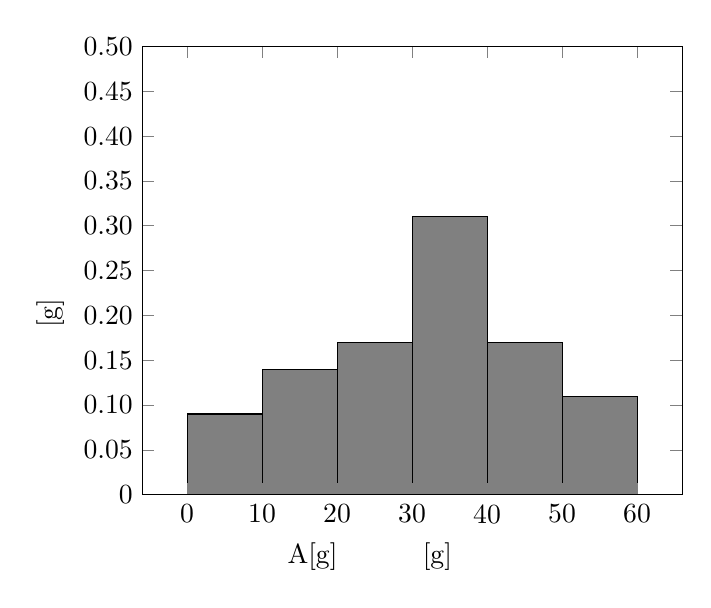
\begin{tikzpicture}
\begin{axis}[ytick={0, 0.05, 0.10, 0.15, 0.20, 0.25, 0.30, 0.35, 0.40, 0.45, 0.50},yticklabels={0, 0.05, 0.10, 0.15, 0.20, 0.25, 0.30, 0.35, 0.40, 0.45, 0.50}, ymax=0.50,ymin=0, area style, xlabel={A\ruby[g]{中学校}{ちゅうがっこう}の\ruby[g]{通学時間}{つうがくじかん}}, ylabel={\ruby[g]{相対度数}{そうたいどすう}}]
\addplot+[ybar interval, mark=no, fill = {gray}, draw = {black}] plot coordinates { (0, 0.09) (10, 0.14) (20, 0.17) (30, 0.31) (40, 0.17) (50, 0.11) (60, 0.00) };
\end{axis}
\end{tikzpicture}

\columnbreak

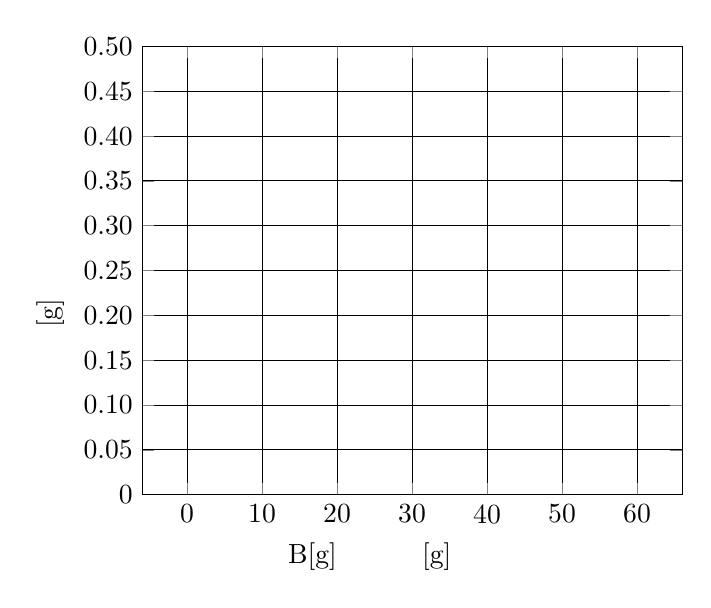
\begin{tikzpicture}
\begin{axis}[ytick={0, 0.05, 0.10, 0.15, 0.20, 0.25, 0.30, 0.35, 0.40, 0.45, 0.50},yticklabels={0, 0.05, 0.10, 0.15, 0.20, 0.25, 0.30, 0.35, 0.40, 0.45, 0.50}, ymax=0.50,ymin=0, area style, xlabel={B\ruby[g]{中学校}{ちゅうがっこう}の\ruby[g]{通学時間}{つうがくじかん}}, ylabel={\ruby[g]{相対度数}{そうたいどすう}}, grid = both, grid style = {black}]
\addplot+[ybar interval, mark=no] plot coordinates { (0, 0) (10, 0) (20, 0) (30, 0) (40, 0) (50, 0) (60, 0) };
\end{axis}
\end{tikzpicture}

\end{multicols}

\begin{center}
\textbf{※ \ruby[g]{問題}{もんだい}は\ruby[g]{次}{つぎ}のページに\ruby[g]{続}{つづ}きます。}
\end{center}

\vfill

\newpage

(\text{\refstepcounter{skaunta}%
\arabic{skaunta}})\hspace{2.5pt}A\ruby[g]{中学校}{ちゅうがっこう}とB\ruby[g]{中学校}{ちゅうがっこう}において、どちらのほうが\ruby[g]{通学時間}{つうがくじかん}が\ruby[g]{長}{なが}い\ruby[g]{傾向}{けいこう}にあるかを\textbf{\ruby[g]{割合}{わりあい}}という\ruby[g]{言葉}{ことば}を\ruby[g]{使}{つか}って\ruby[g]{説明}{せつめい}しなさい。ただし、\ruby[g]{通学時間}{つうがくじかん}が\ruby[g]{長}{ながい}いとは、\ruby[g]{通学}{つうがく}に40\ruby[g]{分以上}{ぷんいじょう}かかることとします。

\vspace{20mm}

(\text{\refstepcounter{skaunta}%
\arabic{skaunta}})\hspace{2.5pt}B\ruby[g]{中学校}{ちゅうがっこう}で\ruby[g]{一人}{ひとり}に\ruby[g]{声}{こえ}をかけて\ruby[g]{通学時間}{つうがくじかん}が40\ruby[g]{分未満}{ぷんみまん}である\ruby[g]{確率}{かくりつ}は、どのくらいだと\ruby[g]{考}{かんが}えられますか。

\vspace{50mm}

\begin{multicols*}{2}

\noindent\fbox{\large\makebox[1em]{\text{\refstepcounter{kaunta}%
\arabic{kaunta}}}} \hspace{1pt}\ruby[g]{右}{みぎ}の\ruby[g]{図形}{ずけい}を、\ruby[g]{直線}{ちょくせん}$l$を\ruby[g]{回転}{かいてん}の\ruby[g]{軸}{じく}として1\ruby[g]{回転}{かいてん}させてできる\ruby[g]{立体}{りったい}の\ruby[g]{体積}{たいせき}を\ruby[g]{求}{もと}めなさい。

%
\begin{flushright}%
\footnotesize{<思・判・表3点>}%
\end{flushright}%


\vfill\null

\columnbreak

\begin{center}
\def\@captype{figure}
\includegraphics[height=35mm]{img/img15.jpg}

\end{center}

\end{multicols*}


\end{flushleft}

\end{document}
